
%--------------- Chapter 2: Literature Survey ---------------%

\chapter{LITERATURE REVIEW}\label{Ch2:Literature Review}
\graphicspath{{Chapter2/Chapter2Figs/}{Chapter2/Chapter2Figs/}}
\section{Introduction}
The general framework of an automated histopathological image classification system, depicted in  Figure \ref{ch1:fig:basic_model1}, mainly composed of two phases, namely  training phase and validation phase.  The first phase is the training phase in which the sampled histopathological images are selected randomly from the database and converted into the feature vectors by an image representation method. The converted feature vectors along with the image labels are fed to the learning model (i.e., classifier) for training. The trained learning model is used in the validation phase in which a histopathological image is selected from the image database and is converted into a feature vector by applying the same image representation method. The obtained feature vector is passed to the trained learning model which predicts the label of the image. Therefore, in the classification of histopathological images, the image representation method plays an important role and the accuracy of a system is highly depends upon its performance. 
\begin{figure}[h!]
%\begin{center}
\centering
     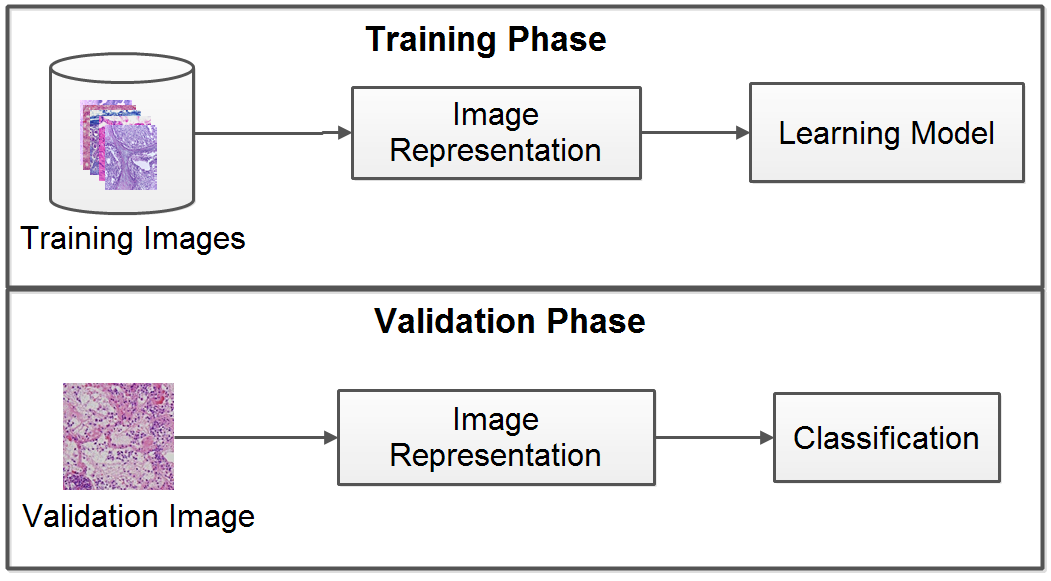
\includegraphics[width=0.8\textwidth]{basic_model1}
   \caption[General work flow of an automated histopathological image classification method]{\fontsize{10pt}{12pt}\selectfont General work flow of an automated histopathological image classification method}
 \label{ch1:fig:basic_model1}
%\end{center}
\end{figure}
On the basis of image representation techniques, the histopathological image classification methods can be divided into three categories, namely statistical-based methods, learning-based methods, and mid-level representation based methods as shown in Figure \ref{ch2:fig:IRM}.
\begin{figure}
%\begin{center}
\centering
     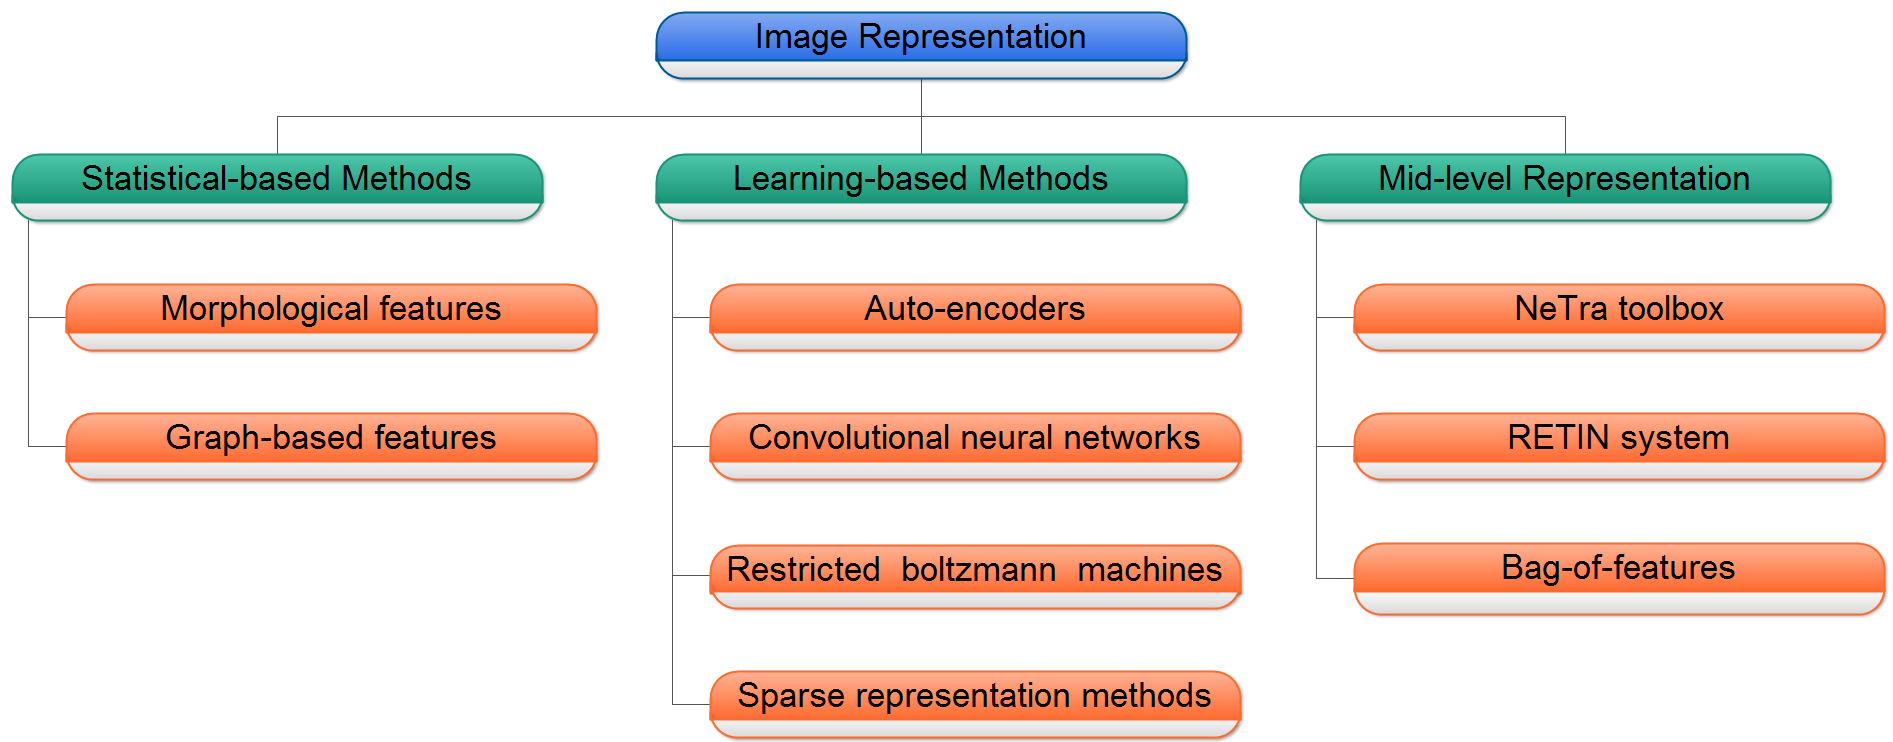
\includegraphics[width=1.0\textwidth]{IRM}
   \caption[Categorization of histopathological image classification techniques based on image representation]{\fontsize{10pt}{12pt}\selectfont Categorization of histopathological image classification techniques based on image representation}
 \label{ch2:fig:IRM}
%\end{center}
\end{figure}


Statistics-based image representation methods extract the low-level or local features from the histopathological images based on pixel-level operations. The features provide enthralling details of the medical image contents for the classification task without the need for segmentation. A low-level feature represents an image region that is different from its instant vicinity \cite{tuytelaars2008}. In statistical-based methods, various characteristics of cells and nuclei are captured like shape, size, color, texture, and distribution of nuclei in small regions or patches \cite{dundar2011}. These features are also called handcrafted features. Various customized feature extraction methods are developed and used to extract the handcrafted features from the images \cite{orlov2008}. For example, to detect the vessel-like patterns in medical images, morphological features have been used \cite{zana2001} while to expose the spatial patterns or structures, various graph-based features have been used such as minimum spanning tree, Delaunay triangulation, query graphs, and others \cite{ozdemir2012}. However, statistical-based image representation methods are not able to express the complex visual morphological structures in histopathological images \cite{qureshi2009} \cite{gutierrez2013}. To overcome this, various learning-based methods have been used for image representation.

The learning-based image representation methods use different machine learning algorithms for automatic feature extraction from the images \cite{zheng2017}. The features represent the images in a more meaningful and collective manner. These method includes auto-encoders \cite{arevalo2014},  CNN (convolutional  neural  networks) \cite{xu2016deep}, RBM (restricted  Boltzmann  machines) \cite{nayak2013}, and sparse  representation \cite{vu2016}. Cruz-Roa et al. \cite{Cruz-Roa2013} presented a deep learning model to automatically detect basal cell carcinoma. It includes an interpretation layer that is used to highlight the patterns for differentiating the normal and cancerous tissues. Furthermore, Arevalo et al. \cite{arevalo2015} used an unsupervised feature learning approach for the analysis of histopathological images. The local patches are represented using different methods like independent component analysis based on topography and reconstruction along with sparse auto-encoders, while for the global representation of the images convolutional neural network is used. Xu et al. \cite{xu2016} applied the stacked sparse auto-encoder to automatically detect the nuclei in breast cancer histopathological images. Further, a deep CNN is trained to learn the features for the segmentation of epithelial and stromal tissues from the breast cancer histopathological images \cite{xu2016deep}.  On the contrary, Srinivas et al. \cite{srinivas2014} introduced a sparsity model for the histopathological images having multiple color channels.  Each image is represented by sparse linear permutations of training samples, having channel-wise constraints. To handle different spatial locations of image objects, a locally robust variant of this method has also been presented.  Further, Vu et al. \cite{vu2016} presented a method for automatic feature learning from the histopathological images having complex morphological structures. The learning is based on class-specific dictionaries having sparsity constraints. The learned dictionaries are further used for the classification and grading of various diseases via histopathological images. However, most of the learning-based methods for image representation are taking high computational cost \cite{gutierrez2013} when applied to complex histopathological images.  Moreover, The patch-selection based methods discussed in \cite{srinivas2014} and \cite{vu2016} are fast but usually failed in identifying inflamed or malignant samples when there is a less malignant area available in the images.

Mid-level feature extraction methods transform the local or low-level feature descriptors into a global representation which is considered as mid-level representations of the images \cite{boureau2010}. As the global features are the descriptors defined by local features, they are generally close to the image-level information.  There are mainly three steps to get the mid-level representation \cite{boureau2010}: (i) local feature extraction, (ii) codebook construction, which is used to find the visual words from the feature set, (iii) encoding, which is generally used to represent each image into a histogram of visual words. Further, a classification algorithm is trained on these histograms.  There are various mid-level image representation methods, available in the literature, and the most widely used methods are NeTra toolbox \cite{ma1999}, RETIN system \cite{fournier2001}, and the bag-of-features (BOF) \cite{caicedo2009}. The first contribution made on the mid-level representation based paradigm is the NeTra toolbox, which uses the unsupervised learning for the construction of the codebook defined over the color point descriptors and the Linde–Buzo–Gray (LBG) algorithm \cite{linde1980} for vector quantization. Further, the RETIN system \cite{fournier2001} uses the self-organized maps \cite{kohonen1982} for generating codebook from Gabor feature vectors. The mid-level representation technique becomes more popular when it is applied in Video Google formalism. Sivic and Zisserman \cite{sivic2003} used the bag-of-features method for the scene and object retrieval in which the features are extracted using scale-invariant feature transform (SIFT) and the codebook construction is done by K-means. Further, Csurka et al. \cite{csurka2004} used this method for the categorization of images. Moreover, Caicedo et al. \cite{caicedo2009} used the bag-of-features method along with the kernel function for the categorization of histopathological images. Kumar et al. \cite{kumar2017} validated that the bag-of-features representations outperform other representation methods for histopathological image classification. Therefore, in this work, bag-of-features methods are studied for histopathological image classification. The following section presents the state-of-art methods used in various phases of the BOF method for histopathological image classification.
  

\section{Bag-of-Features Method}\label{subsubsec:BOF}

In literature, the BOF method has emanated as a convenient mechanism for histopathological image classification. It generally consists of four prime phases:  (i) feature extraction,  used to detect and represent the keypoints as feature descriptors, (ii)  codebook construction, used to cluster the feature descriptors for generating the visual words, (iii) feature encoding in which each image is represented in a form of visual words, and (iv) classification phase which trains a classifier using the generated form of images along with the corresponding labels. The detailed survey of each phase of the bag-of-features method is presented in the following sections.

\subsection{Feature Extraction}\label{subsec:Feature Extraction}

In the BOF method, each input image is represented as a pool of local features by a feature extraction method. The feature extraction phase detects features from an image and represents them as a feature descriptor. 

The process of identification of local features, such as corners, blobs, edges, and interest points in an image, is called feature detection. A good feature detection method should generate relevant and distinct features.  Once the features are detected from an image, it is converted to a feature descriptor by taking the measurements from the region centered at the interest point. In the BOF method, feature extraction methods can be categorized into two categories, namely interest point based features and learned features. Interest point detection based methods are based on the analysis of corner points in different scale spaces. These methods can further be categorized into two types, namely partial differential equation (PDE) based methods and template-based methods. The PDE based methods use partial differentiation on Gaussian scale spaces, for example  difference of Gaussian (DoG) \cite{raza2011}, Hessian-Laplacian \cite{orting2018}, SIFT \cite{lowe2004}, speeded-up robust features (SURF) \cite{spanhol2016}, etc. Moreover, template-based methods use decision tree and binary comparison for extracting the features like binary robust invariant scalable keypoints (BRISK) \cite{leutenegger2011}, fast retina keypoints (FREAK) \cite{alahi2012}, and oriented features from accelerated segment test and rotated binary robust independent elementary features (ORB)\cite{spanhol2016}. The learned features are the deep features extracted from the images which are generally high-level abstraction obtained from raw images. Some of these methods available in literature are deep neural networks (DNN) \cite{bar2015}, stacked sparse auto encoder (SSAE) \cite{xu2014}, and CNN \cite{cruz2013}. A brief overview of various feature extraction methods used for histopathological images are presented in Table \ref{ch2:Tab:features} \cite{li2015}.


\begin{table}
\renewcommand{\arraystretch}{1.5}
\centering
\caption[Categorization of features extraction methods used in bag-of-features]{\fontsize{10pt}{12pt}\selectfont Categorization of features extraction methods used in bag-of-features \cite{li2015}}
\label{ch2:Tab:features}
\footnotesize{
\begin{tabular}{p{2.8cm}|p{3.5cm}|p{4cm}|p{3.5cm}}
     \hline
    \textbf{Category}  & \textbf{Classification} &  \textbf{Comments} & \textbf{Methods}\\
     \hline 
    Blob Detection (Interest Point) &  Partial Differential Equations (PDE) based & Use the PDE on Guassian scale spaces &  DoG \cite{polakowski1997}, Hessian-Laplacian \cite{orting2018}, SIFT \cite{lowe2004}, SURF \cite{bay2008}\\

 & Template based & Decision tree and binary comparison methods are used; Computationally fast & BRISK \cite{leutenegger2011}, FREAK \cite{alahi2012}, ORB \cite{rublee2011}\\

Learned Features & Deep Features &  High-level abstractions obtained from raw images &DNN \cite{bar2015}, SSAE \cite{xu2014}, CNN \cite{cruz2013} \\
\hline
\end{tabular}
}
\end{table}
In this work, the interest point based feature detection methods are studied.
An interest point in an image is a robustly detected and well-defined location, also known as keypoint which can be a corner point, an isolated point, and a point on a curve. In literature \cite{durand2013}, most of the corner detection methods are used to find the interest points in an image.  The Harris corner detector \cite{harris1988} detects the corner points more precisely by the use of first derivatives and considering the neighborhood information.  These points are known as interest points as these are illumination and rotation invariant and robust to the noise. However, the interest point is not invariant to large scales \cite{schmid2000}. To overcome this,  the Harris-laplace detector \cite{mikolajczyk2002} has been introduced which considers different scales by the use of  laplacian transform. However, the number of points returned by the Harris-laplace detector is very less. Therefore, another version of the Harris-laplace detector has been introduced with less strict criteria \cite{mikolajczyk2005}. Furthermore, for the inclusion of affine-invariant patches the Harris-Affine detector can be used \cite{mikolajczyk2004}. The detailed comparative analysis of these methods along with other corner detectors is provided by Mikolajczyk et al. \cite{mikolajczyk2005}. 

Furthermore, SIFT \cite{lowe2004}, SURF \cite{bay2008}, and ORB \cite{rublee2011} features are the most widely used method for feature detection and description. SIFT  is a method to detect and describe the low-level features from the digital images. First, it finds some interest points and then represents them in a quantitative manner known as descriptors. These descriptors are robust to scale, rotation, and illumination conditions. Irshad et al. \cite{irshad2013} introduced an automated method for the detection of mitosis to assist the pathologists. The color spaces are distinguished by analyzing the combined pattern of texture features, namely SIFT along with the run-length and co-occurrence features. These features are then fed to the SVM (support vector machine) for the classification purpose. Further, Raza et al. \cite{raza2010} used scale invariant features in the BOF framework for the identification of subtypes in RCC (renal cell carcinoma).  Caicedo et al. \cite{caicedo2009} also used the BOF method with SIFT for feature detection and description to classify histopathological images automatically.  Raza et al. \cite{raza2011} studied and analyzed the rotation and scale in-variance behavior in the  BOF method for the classification of histopathological images of RCC.


SURF \cite{bay2008} is a fast and efficient interest point detector method which uses the integral image for the convolutions. The method works in three phases, namely keypoint detection, description, and matching. Yang et al. \cite{yang2013} solved the problem of image stitching in biomedical research about the whole sections or larges areas. The proposed method considers the SURF method for feature extraction in a fast and efficient manner. Sanghavi and Agaian \cite{sanghavi2016} proposed an automated method for the classification of histopathological images of prostate cancer based on the bag-of-features method. For feature extraction, a comparative analysis is presented between SURF and SIFT features based bag-of-features method. SURF returns higher sensitivity as compared to SIFT-based bag-of-features.  Wand and Chen \cite{wang2013} addressed the problem of image alignment in X-ray images and tissue images and compared it with five other methods, namely TrackEM2, UnwarpJ, BUnwarpJ, mutual information, and SURF. The proposed method shows better results on both of the datasets.


ORB \cite{rublee2011} uses oriented FAST \cite{tuzel2006} method as a high speed corner detector and the detected corned are represented by a variant of BRIEF descriptor, i.e., binary robust independent elementary features  descriptor \cite{calonder2011}. Davidson et al. \cite{davidson2018} introduced a new method for stitching the images with the use of ORB descriptors, along with good enough transformation and local sensitivity hashing for fast processing. The proposed method is applied to study adaptive optics ophthalmoscopy automatically and efficiently. Further, Adel et al. \cite{adel2018} used ORB for extracting the features from microscopic images of Oral Epithelial Dysplasia and fed these features to SVM for the automated grading of disease. 

Moreover, SIFT and SURF features are robust to scale, rotation, and illumination changes while ORB is a computationally fast method. However, due to complex morphological structures of histopathological images, these methods generate high dimensional feature vectors.


\subsection{Codebook Construction}\label{subsec:Codebook Construction}

The second phase of the BOF method is the codebook construction in which the extracted features are divided into different clusters to find the visual words. The pool of visual words is known as a codebook. In literature, various clustering methods are used for codebook construction in BOF, mentioned in Table \ref{Tab:clustering}, which can be grouped into three classes, namely hierarchical methods, partitional methods, and meta-heuristic based methods. 

\begin{table}
\renewcommand{\arraystretch}{1.5}
\caption [Various codebook construction methods used in the bag-of-features]{ \fontsize{10pt}{12pt}\selectfont Various codebook construction methods used in the bag-of-features \cite{jurie2005}}
\label{Tab:clustering}
\centering
    
\footnotesize{
\begin{tabular}{p{3cm}|p{4cm}|p{7cm}}

     \hline
    
    \textbf{Category} &\textbf{Methods}  &  \textbf{Comments}\\
     \hline 
    Hierarchical methods & Agglomerative clustering, Mean shift  & These methods can not be applied to large datasets or histology images due to high computational cost. \\

Partitional methods & K-means, FCM, GMM  & Generates non-uniform coding (biased towards dense regions); \newline Non robust; \newline Optimal codebook size (K) is unambiguous.\\


Meta-heuristic based methods & PSO, GSA, WOA & Used to find optimal visual words based on some objective function defined over compactness and separation; \newline Computationally expensive. \\


\hline
\end{tabular}
}
\end{table}

\begin{itemize}
\item \textbf{Hierarchical Clustering:}
In hierarchical clustering, the grouping of data at different similarity levels is performed which is schematized by a tree-like structure termed as a dendrogram. Generally, the hierarchical splitting follows two approaches, namely divisive and agglomerative \cite{saxena2017review}. In divisive clustering, recursive hierarchical data splitting is performed in a top-down fashion to generate the clusters. All the data items belong to a single cluster initially and  further divided into various small clusters until a terminating condition is satisfied or until each data item forms its cluster. Divisive clustering (DIVCLUS-T) \cite{chavent2007divclus} and divisive hierarchical clustering with diameter criterion (DHCDC) \cite{guenoche1991efficient} are popular methods of this category. On the other side, the agglomerative clustering is performed in the bottom-up fashion where data points are merged hierarchically to produce clusters. Initially, each data item defines itself as a cluster which is further merged into bigger clusters, until a termination criterion is meet or until a single cluster is formed consisting of all the data items. Some popular agglomerative methods are balanced iterative reducing and clustering using hierarchies (BIRCH) \cite{zhang1996birch}, chameleon \cite{karypis1999chameleon}, and clustering using representatives (CURE) \cite{guha1998cure}.

Meijnen et al. \cite{meijnen2008} used the hierarchical clustering method for dividing the in-situ ductal carcinoma breast cancer images into two major groups and each major group is further divided into five sub-classes based on six markers. The proposed method is used to investigate gene expression profiling.  Bhargava et al. \cite{bhargava2006} developed a system for automated spectroscopic analysis of tissue images. For the segmentation of tissue images, hierarchical clustering methods are used and the combination of tissue microarray analysis with Fourier transform of spectroscopic images are used for high throughput analysis. Furthermore, Pourahmad et al. \cite{pourahmad2016} developed a framework for the automated grading of colorectal cancer with the use of hierarchical clustering and partitional clustering approaches. As per the experimental analysis, hierarchical clustering outperforms other considered clustering methods.

Generally, hierarchical methods employ a greedy approach and do not reconsider a data point after it has been assigned to a cluster. This results in lacking the capability of correcting the misclassified data point. Therefore, these methods lack robustness, especially in the case of noise and outliers. They do not intend to optimize an objective function while forming the clusters. Moreover, they perform poorly when clusters are overlapping. While generating clusters for a particular problem, knowledge about the number of clusters is required. Moreover, the formation of spherical clusters and the reversal of the hierarchical structure are distorted \cite{xu2005survey}. Additionally, one of the major issues while clustering data through a hierarchical approach, especially on high-dimensional dataset like image, is the time complexity. The time complexity of hierarchical methods is very expensive which is approximately defined as $O(n^3)$ \cite{saxena2017review}, where $n$ corresponds to the number of data points. Hierarchical clustering methods, such as agglomerative clustering \cite{leibe2006} and mean shift \cite{georgescu2003}, cannot be applied to large datasets or histology images due to high computational cost. Therefore, to overcome this limitation, partitional clustering methods are preferred which are discussed in the following section. 

\item \textbf{Partitional Clustering:} It is relatively quite popular and preferred over the hierarchical clustering, especially for large datasets, due to its computational efficiency \cite{bouguettaya2015efficient}. In this type of clustering method, the notion of similarity distance is usually used as the measurement parameters. Thus, partitional clustering is the process of dividing the data into clusters according to the considered objective function such that similar data points  belong to one cluster and dissimilar data points in other clusters. To achieve this, the distance of each data point is measured from every cluster center and is allocated to that cluster which is nearest. Moreover, in partitional clustering, the general notion of the objective function is the minimization of the within-cluster similarity criteria which is usually computed by Euclidean distance. The objective function expresses the goodness of each formed cluster and returns the best representation from the generated clusters. Moreover, these methods surely assign data point with a cluster even if it is quite far from the respective cluster centroid which, sometimes, results in distortion of the cluster shapes or false results, especially in the case of noise or outlier \cite{xu2005survey}. There are two classes of partitional clustering methods, namely soft and hard clustering methods. 

Soft clustering methods assign each data to either two or more clusters with a degree of belongingness (or membership) iteratively. The degree of belongingness illustrates the level of association among data more reasonably.  Some popular methods are fuzzy c-means (FCM) \cite{bezdek1973cluster}, fuzzy c-shells (FCS) \cite{dave1992adaptive}, and mountain method \cite{yager1994approximate}. In FCM, each cluster is considered as a multidimensional hypersphere and defines the distance function accordingly. Mountain method uses the mountain function to find the cluster centers. Particularly, FCM is the most widely used and popular method of this approach.

Hard clustering methods partition the data into disjoint clusters according to the objective function. Generally, the objective function is the sum of squared Euclidean distance between data and associated centroid which is to be minimized. Usually, the center of the clustered data is considered as the centroid of the clusters in these methods. Moreover, in contrast to soft clustering, hard clustering assigns data to a single cluster only i.e., each data will have the degree of belongingness as either 0 or 1. One of the popular hard clustering methods is K-means \cite{wang2015}. In K-means based methods, the cluster center is cosidered as the mean of all the data points assigned to the corresponding cluster. This is iteratively continued until some defined convergence criterion is met. K-means method has the time complexity of $O(nkt)$ \cite{saxena2017review} where, $t$ corresponds to the maximum iterations. This method is biased towards initial cluster centroids and usually gets trap into local minima. Moreover, solutions vary with the number of clusters. 

Rueda et al. \cite{rueda2012bag} used K-means clustering for codebook construction in the BOF method for the classification of magnetic resonance images of Alzheimer's disease. Cruz-Roa et al. \cite{cruz2011} used the BOF method for the representation of visual content in histopathological images. K-means is used to find different visual words in the BOF method. Wiliem et al. \cite{wiliem2013classification} used K-means clustering for generating the codebook from SIFT-based descriptors and used them for the classification of immunofluorescence images of human epithelial cells. Avni et al. \cite{Avni2010} generated the patch based visual words for the categorization of the X-ray images for automated retrieval. Further, Stanciu et al. \cite{Stanciu2014} used the BOF method along with K-means for codebook generation for the diagnosis of liver fibrosis by excitation microscopy of two photons. 

Therefore, various partitional clustering methods, used in the bag-of-features, are K-means, FCM, and GMM \cite{saygili2015}. Some of them are discussed above. However, these methods are biased towards dense regions and may generate non-uniform coding. 

\item \textbf {Meta-heuristics based Clustering:} This category involves the use of meta-heuristic approaches to obtain optimal clusters, especially in the case of images. These approaches use random solutions that are updated according to defined optimality criteria known as objective function \cite{zhang2011image}. A meta-heuristic algorithm computes the objective function value by using the generated solutions. A meta-heuristic algorithm must be efficient so that the optimal solution can be reached.  Broadly, the algorithms of this category belong to the class of optimization algorithms which correspond to a set of algorithms that can solve computationally hard problems like NP-complete problems. An NP-complete problem is a problem for which there exists no deterministic algorithm that can provide the exact solution in polynomial time. There exist several optimization algorithms in the literature, however, no single algorithm is efficient in solving every problem as stated by No Free Lunch Theorem \cite{wolpert1997}.

Researchers have proposed many such algorithms and their variants based on the inspiration from nature to provide an efficient and optimal solution. Over the last three decades, more than sixty meta-heuristic algorithms have been proposed. As these algorithms are inspired by nature, each algorithm mimics particular natural phenomena that may belong to evolutionary, physical, or biological. Researchers are continuously working to improve the existing algorithms and also proposing new algorithms that are giving competitive results as compared to the existing algorithms present in the literature.  Two common aspects that are often found in these algorithms are exploration and exploitation \cite{yang2014}. Exploration represents the diversification in the search space wherein the existing solutions are updated to explore the search space. This helps in exploring the new solutions, prevents the stagnation problem, and responsible for achieving the global solution. The exploitation, which corresponds to the intensification of the current solution, performs the local search around the currently generated solutions. In this, the goal is to exploit the search space and responsible for convergence to the optimal solution. Generally, meta-heuristic algorithms may broadly be classified into two categories, namely evolutionary and swarm algorithms.

Evolutionary-based algorithms are based on evolution theories such as Darwin evolutionary theory. The evolutionary algorithms work on the principle of generating better individuals with the course of generation by combining the best individuals of the current generation. The genetic algorithm (GA) \cite{maulik2000genetic} is an evolutionary algorithm based on the evolution of natural species. It implements the exploration and exploitation through the mutation and crossover operators respectively. Another biological process based evolutionary algorithm is evolutionary strategy \cite{babu1994clustering} which performs recombination and mutation with equal probability and uses multiple parents to accord an offspring. Differential evolution (DE) is another popular evolutionary algorithmic introduced by Storm et al. \cite{storn1997}. Simon \cite{Simon2008} presented biogeography-based optimization (BBO) which is based on the immigration and emigration of the species between the islands of natural biogeography. Baluja \cite{dasgupta2013evolutionary} proposed the probability-based incremental learning algorithm which manages only statics of the population rather than managing the complete population.

Swarm-based algorithms behave like the swarm of agents such as fishes or birds to achieve optimal results. Kennedy \cite{kennedy2011} proposed the particle swarm optimization (PSO) which mimics the swarm behavior of birds or fishes for searching the food. Ant colony optimization (ACO) imitates the ant's behavior for finding paths \cite{dorigo2006}. Gravitational search algorithm (GSA), introduced by Rashedi et al. \cite{rashedi2009}, is an algorithm based on Newtonian laws of gravity and motion. Hosseini \cite{shah2009} proposed an intelligent water drop algorithm based on the flow of rivers, as rivers often follow the shortest path while flowing from source to destination. Further, Wang et al. \cite{wang2014} proposed the hybrid krill heard algorithm to overcome the problem of poor exploitation capability of the krill herd algorithm.  Bansal et al. \cite{Bansal2014} introduced spider monkey optimization (SMO) that mimics the behavior of spider monkeys. Furthermore, Mirjalili \cite{mirjalili2015} proposed an ant-lion based optimizer that imitates the behavior of ant-lions. Mirjalili \cite{mirjalili2015a} also introduced the moth-flame optimization, which simulates the death behavior of moths, in which the movement of the agent is based on the transverse orientation based navigation of moths. Some recent swarm algorithms are multi-verse optimizer \cite{mirjalili2016multi}, galaxy-based search algorithm \cite{shah2011principal}, small-world optimization algorithm \cite{du2006}, and ray optimization \cite{kaveh2012new}.

The various meta-heuristic algorithms can provide promising results for unfolding the   clustering problem. Generally, these clustering-based methods are better than other clustering methods in terms of independence from the initial parameter settings and return global optimal solution \cite{jose2016automatic}. As these methods ensure a better solution, their use in clustering has been prominent in the literature. The basic approach to emerge meta-heuristics based clustering algorithm was introduced by Selim and Alsultan \cite{selim1991simulated}, using simulated annealing. After that, Bezdek et al. \cite{bezdek1994genetic} presented a genetic algorithm based data clustering method that was the first evolutionary based method of data clustering.  The first, swarm-based clustering method was developed by Lumer et al. \cite{langham1999using} using ant colony optimization.  
\begin{algorithm}[h!]
\caption{Meta-heuristic based clustering method}
\label{algo:metah}
\setstretch{1.5}
{\footnotesize
\begin{algorithmic}
\STATE\textbf{Input:} Initialize the number of clusters to be formed.
\STATE\textbf{Output:} Clustered data.
\STATE Choose a population of random individuals where, each individual corresponds to a cluster center.
\WHILE{clustering condition is not satisfied or centers do not change}
\STATE Calculate the fitness value of each solution through the considered objective function;
\STATE Update the solution according to the meta-heuristic algorithm;
\STATE Assign each data point to the nearest cluster center;
\ENDWHILE
\end{algorithmic}
}
\end{algorithm}

Meta-heuristic based clustering methods like BBO \cite{Pal2018}, GSA \cite{Mittal2019}, and whale optimization algorithm (WOA) \cite{Tiwari2019} are used to find optimal visual words based on some objective functions defined over compactness and separation. Mittal and Saraswat  \cite{Mittal2019} proposed a modified version of the  BOF method by generating the optimal visual words using GSA. The proposed methods is validated against the K-means clustering based BOF method for the categorization of tissue images. However, these methods  have high computational cost when applied to complex histopathological images. The pseudo-code for a meta-heuristic based clustering method is presented in Algorithm \ref{algo:metah}.
\end{itemize}

\subsection{Feature Encoding}\label{subsec:Feature Encoding}

The third phase of the BOF method is feature encoding in which each image is encoded in terms of visual words by a feature encoding method.  Each image is encoded as a coding vector of size ($k$), where $k$ represents the count of visual words. Based on the properties of the encoding method, they are divided into three main categories, namely voting, reconstruction, and super-vector based encoding methods \cite{peng2016}. The brief descriptions of these methods are also provided in Table \ref{Tab:encoding}. 

\begin{table}
\renewcommand{\arraystretch}{1.5}
\caption[Various types of feature encoding methods]{\fontsize{10pt}{12pt}\selectfont Various types of feature encoding methods  \cite{huang2014, peng2016}}
\label{Tab:encoding}
\centering
\footnotesize{
\begin{tabular}{p{2.5cm}|p{5cm}|p{7.2cm}}
     \hline
    \textbf{Type} &\textbf{Methods}  &  \textbf{Comments}\\
     \hline 
    Voting based & HV \cite{sivic2003}, SA \cite{Gemert2010}, LSA \cite{Liu2011}, Salient Coding \cite{Huang2011salient},  & Based on the formation of histograms which represent the distribution of visual words\\

Reconstruction based & OMP \cite{Tropp2007}, Sparse coding  \cite{Yang2009}, LLC \cite{Yu2009}, LCC \cite{Wang2010} &  Each feature should be reconstructed by the visual words by applyin some constraints and solving least-sqaure optimization problem \\

Super vector based & LTC \cite{Yu2010}, SVC \cite{Zhou2010}, Fisher Vector \cite{Perronnin2010}, VLAD \cite{Jegou_2012} & Gaussian mixture model is used for estimating the feature distributions which contain means, co-variance, and weights of Guassian ditributions \\
 \hline
\end{tabular}
}
\end{table}


\begin{itemize}
\item \textbf{Voting-based methods:} 
In the voting-based method, each feature descriptor cast their vote for any of the codeword based on some rules or strategy. In response to these voting, a coding vector of $k$ dimensions is created, which is known as a codeword. The collection of codewords is used to make the whole codebook. The most commonly used methods in this category are hard voting (Vector Quantization (VQ)) \cite{sivic2003}, kernel codebook encoding (KCB), soft assignment (SA) \cite{Gemert2010}, localized soft assignment (LSA) \cite{Liu2011}, and salient coding \cite{Huang2011salient}.

For each feature vector $f$, the voting value  for the visual word $v$ can be calculated as a function of $f$,  namely $c(i)=\phi(f)$. The formulation of $\phi(f)$ is different for each type of encoding method. In hard voting methods, each feature can cast the vote to its nearest codeword. Therefore, the formulation of $\phi(f)$  is defined as follows:

\begin{equation}\label{ch2:eq:f}
\phi(f)=\begin{cases}1 & \arg min_j ||f-v_j||_2, \\0 & otherwise,\end{cases}
\end{equation}
The VQ methods are computationally efficient but sometimes it may loss some information. As the resolution to this problem, soft coding methods are introduced which are also known as soft assignment based methods. In soft assignment technique, each feature must cast their vote to every visual word with some normalized weight (i.e., $\phi(f)=w_i$. This normalized weight ($w_i$) of $i^{th}$ feature vector $f$ for $j^{th}$ visual word ($v_j$) is defined in Eq. (\ref{ch2:eq:wi}).
\begin{equation}\label{ch2:eq:wi}
w_i=\frac{\exp(-\beta\parallel f- v_j\parallel^2_2)}{\sum_{j=1}^k\exp(-\beta\parallel f- v_j\parallel^2_2)}
\end{equation}
Furthermore, Liu et al.  \cite{Liu2011} proposed a variant of soft assignment methods, namely localized soft assignment in which a feature can only votes for its $k-$nearby codewords. The normalized weight formulation is modified by inducing an indication function ($I(f,v_j)$) for searching the k-nearest neighbor ($N_k$) members of $f$. The indication function and modified normalized weight is given in Eq. (\ref{ch2:eq:mwi}) and Eq. (\ref{ch2:eq:I}) respectively.
\begin{equation}\label{ch2:eq:mwi}
w_i=\frac{I(f,v_j)\exp(-\beta\parallel f- v_j\parallel^2_2)}{\sum_{j=1}^k\exp(-\beta\parallel f- v_j\parallel^2_2)}
\end{equation}
\begin{equation}\label{ch2:eq:I}
 I(f,v_j)=\begin{cases}1 &  v_j \in N_k(f), \\0 & otherwise,\end{cases}
\end{equation}
Further, salient coding is another type of hard vector quantization method. Each feature calculates its weighted vote based on the difference between the nearest visual word and the other $k-1$ nearest visual words \cite{Huang2011salient}. 
The visual description of each voting based methods is depicted in Figure \ref{ch2:fig:votingbasedmethods}.

\begin{figure}[h!]
\centering
\subfigure[VQ]{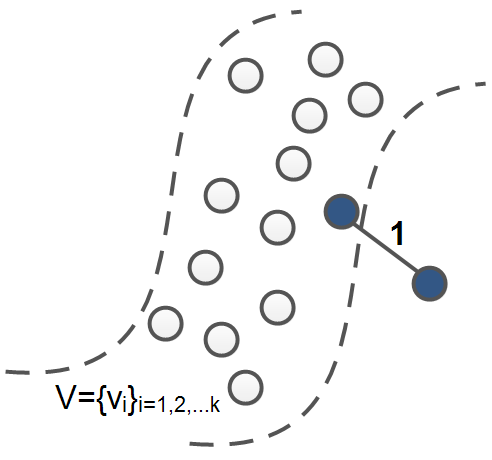
\includegraphics[width=0.22\textwidth]{VQ}}
\subfigure[SA]{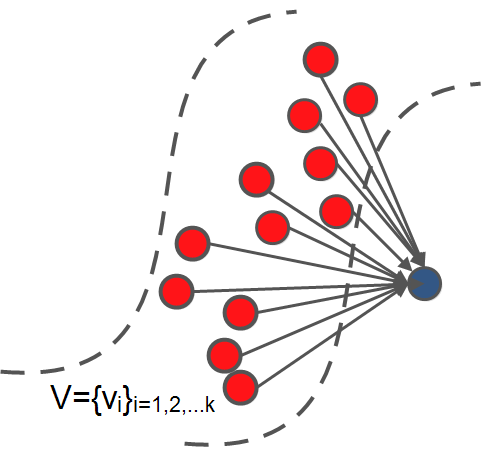
\includegraphics[width=0.22\textwidth]{SA}}
\subfigure[LSA]{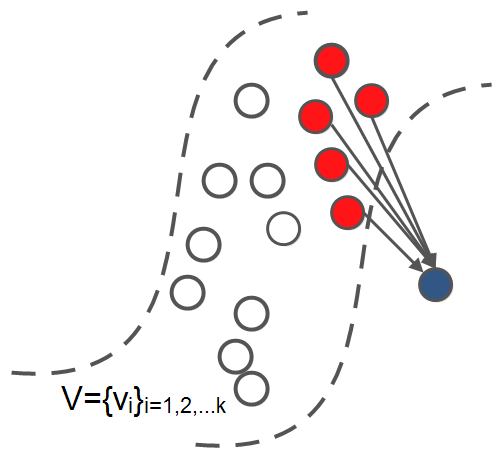
\includegraphics[width=0.22\textwidth]{SA-k}}
\subfigure[Salient Coding]{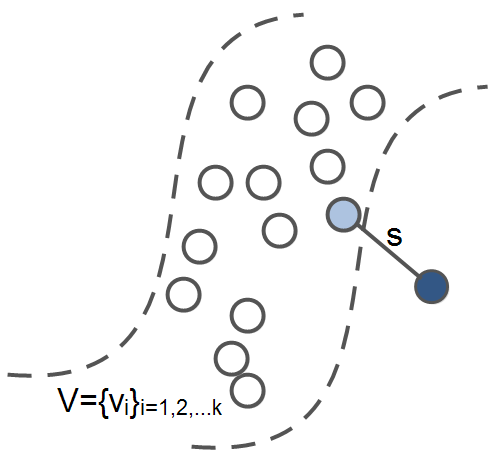
\includegraphics[width=0.22\textwidth]{SC}}
 \caption[Visual description of voting based methods]{\fontsize{10pt}{12pt}\selectfont Visual description of voting based methods \cite{peng2016}}
    \label{ch2:fig:votingbasedmethods}
\end{figure}

\item \textbf{Reconstruction-based methods:} 
In reconstruction-based encoding methods, code $c$ is formulated in the reconstruction or decoding perspective. The  $i^{th}$ input descriptor can be decoded from the code $c$ with the objective of minimum reconstruction error. The objective is equated in Eq. (\ref{ch2:eq:c}) with a regularization component ($\Psi$).
\begin{equation}\label{ch2:eq:c}
\arg min_{c} {\parallel f - V_c ||}^2_2 + \lambda \Psi(c),
\end{equation}
where $\Psi(c)$ corresponds to the properties of $c$ while $\lambda$ is the balancing parameter between the reconstruction error and $\Psi(c)$. 

Some prominent reconstruction methods  are sparse coding (SPC) \cite{Yang2009}, orthogonal matching pursuit (OMP) \cite{Tropp2007}, local coordinate coding (LCC) \cite{Yu2009}, and locality-constrained linear coding (LLC) \cite{Wang2010}. 

OMP method constrains $\Psi(c)$ with $l_0$ - norm \cite{Bruckstein2009} which is defined in Eq. (\ref{ch2:eq:psi}) and follows sparse encoding. However, the $l_0$-norm is non-convex, therefore, this problem requires some heuristic approach for the solution. 
\begin{equation}\label{ch2:eq:psi}
\Psi(c)=  \sqrt[0]{\sum_i f_i^0}
\end{equation}
This non-convexity is relaxed by SPC method with the use of $l_1$-norm \cite{lee2007efficient} which results in obtaining global optimal solution. The modified constraint function of using  $l_1$-norm is given in Eq. (\ref{ch2:eq:mpsi}).
\begin{equation}\label{ch2:eq:mpsi}
\Psi(c)=  \sum_i f_i
\end{equation}
In the SPC and OMP methods, locality is not defined theoretically, but it is measured based on the empirical analysis \cite{Yu2009}. Therefore, Yu et al. \cite{Yu2009} proposed a variant of SPC, namely LCC wherein locality of the encoding is encouraged instead of sparsity. Moreover,  Wang et al. \cite{Wang2010} introduced a faster version called LLC, for the large scale problems.

\item \textbf{Super-vector based methods:}  
In super-vector based encoding methods, high order statistics are aggregated to obtain high dimensional encoding representation. The popular methods of this category are super vector coding (SVC) \cite{Zhou2010}, local tangent-based coding (LTC) \cite{Yu2010}, vector of locally aggregated descriptors (VLAD) \cite{Jegou_2012}, and fisher vector (FV) \cite{Perronnin2010}.  
In LTC \cite{Yu2010}, encoding is formulated in terms of manifold approximation and intrinsic dimensionality where, the non-linear feature manifold is approximated as a local linear function according to the Lipschitz smooth condition and this linear function consists of lower intrinsic dimensionality which is obtained through principal component analysis (PCA). Further,  Zhou et al. \cite{Zhou2010} proposed a simplified version of LTC, known as  SVC, in which vector quantization is employed instead of PCA. Moreover, another super-vector based encoding scheme is fisher vector which is based on fisher kernel \cite{jaakkola1999exploiting} and leverages both generative and discriminative approaches. This method is used for the categorization of large scale images \cite{Perronnin2010}. Further,  Jegou et al. \cite{Jegou_2012} proposed a complex and restricted version of FV which keeps only first-order statistics for encoding. 

 Wiliem et al. \cite{wiliem2013classification} proposed a new automated method for the recognition of human epithelial cells which represents each image into the codebook descriptor vectors having dual regions and feds these descriptors to the nearest convex hull method for the classification. The codebook descriptors are generated by various encoding methods, namely vector quantization, sparse coding, and soft assignment.   Zhou et al. \cite{Zhou2014} developed a learning model based on the multispectral sparse coding based on the convolutions for the classification of histology tissue sections. Further, Nayak et al. \cite{nayak2013} also used sparse codes for finding the unique patches such as necrosis and viable tumor from the histology tissue sections.
 
In histopathological image analysis, voting-based encoding methods are widely used for the encoding of images. Nowakova et al. \cite{Nowakova2018} presented a new method of vector quantization by the inclusion of fuzzy s-trees and fuzzy signatures to resolve the problem of medical image retrieval especially mammography images. Diamant et al. \cite{Diamant2017} used vector quantization based encoding method in the BOF and relevant visual word per task is selected based on mutual information for the automated classification of medical images.  Han et al. \cite{Han2015} proposed a hierarchical vector quantization method to detect pulmonary nodules in CT images. The high-level and low-level VQ methods are responsible to detect lung segments and inter nodule candidate segments respectively.   Another variant of VQ, namely learning vector quantization (LVQ) is presented by Dieterle et al. \cite{Dieterle2003} for the evaluation of urinary nucleoside. The LVQ method has been compared with SVM and neural networks. Mattfeldt et al.  \cite{mattfeldt2004classification} applied the LVQ method to classify prostate incidental carcinoma. Further, another version of vector quantization is introduced by Hipp et al. \cite{Balis2011} which attains better performance as compared to standard VQ for the pattern recognition in pathological images. 

\end{itemize}


\subsection{Classification}\label{subsec:Classification}

A classifier is used to categorize or identify the image labels or components based on the features extracted from these images. The richness and quality of feature descriptors affect the performance of the classifiers. Histopathological image classification is a complex process for the machine or computer system which motivates the research community to study and analyze this field in perspective of machine intelligence. 

\begin{table}[ht!]
\renewcommand{\arraystretch}{1.3}
\caption[Popularly used classification methods for histopathological image classification]{Popularly used classification methods for histopathological image classification}
\label{ch2:Tab:classification}
\centering
\footnotesize{
\begin{tabular}{p{3.5cm}|p{8.5cm}|p{2.5cm}}
            \hline
              \textbf{Classifier}& \textbf{Details} &  \textbf{Applications} \\
             \hline
            Random Forest &  The prediction is done based on the majority voting of different decision trees  &  \cite{spanhol2016} \cite{sommer2012learning} \cite{Cruz-Roa2014}\\
            Logistic Regression  &  The score value is calculated based on the linear fucntion for the prediction of the target class & \cite{xu2016} \cite{hou2016} \cite{Wang2014a}     \\
      
            Support Vector Machine &  Data is classified by the defined hyperplane and new image is categorized based on hyperplane & \cite{Wang2016} \cite{Zhang2015} \cite{doyle2008}   \\
            
            Linear Discriminant Analysis & The separation between two or more classes is found based on the linear combination of features & \cite{Sertel2008} \cite{Sertel2008a} \cite{Esgiar1998}     \\
            
            Bayesian Classifier &  Based on the conditional probability model where the classification is  probabilistically related to the observed samples  & \cite{Huang2009} \cite{Zhou2015} \cite{Naik2008} \cite{Doyle2012} \\
            \hline
        \end{tabular}
}
\end{table}
In the last phase of the BOF method, a classifier is trained using encoded images and their corresponding labels. After the training of a classifier, it is used to test the unknown encoded images.  Table \ref{ch2:Tab:classification} enlists some of the popular classifiers used in the literature \cite{gurcan2009} along with their application to the histopathological image classification.


\section{Research Gaps and Objectives}
After reviewing the literature, following sections discuss the identified research gaps and research
objectives.
\subsection{Research Gaps}
\begin{enumerate}
\item  Histopathological images contain various morphological variabilities and structures, due to which high dimensional keypoint descriptors are generated. This makes codebook construction computationally expensive and prompts to generate irrelevant visual words. No method has been reported to select the prominent keypoints in the BOF method for histopathological images;

\item The generated visual words are biased towards the densest regions in descriptor space and due to which other informative regions could not be encoded; 

\item Existing meta-heuristic based visual word generation methods are computationally expensive, and 
\item Existing feature encoding methods consider only a single image feature to encode an image. 

\end{enumerate}



\subsection{Objectives}
After examining the research gaps, the following research objectives are defined:
\begin{enumerate}
    
    \item A new keypoint selection method has to be designed and developed to find discriminative and relevant features for codebook construction;

    \item An efficient meta-heuristic based codebook generation method has to designed and developed to reduce the effect of dense regions of histopathological images;
    
    \item A computationally efficient and effective codebook generation method has to be designed and developed for finding the relevant visual words, and
    

    \item An efficient feature encoding method has to be designed and developed by incorporating the merits of two different features descriptors for the better image representation.
    
\end{enumerate}


\section{Summary}\label{Ch2:sec:Summary}
In this chapter, different types of image representation methods for histopathological image classification have been reviewed. The BOF method is one of the popular image representation techniques which performs better on histopathological images. There are four main phases of the BOF method, namely feature extraction, codebook construction, feature encoding, and classification.  The popular feature extraction methods, like SIFT and SURF, are invariant to rotation, light illumination, and scaling but, these methods generate high dimensional feature vectors when applied on histopathological images. Therefore, there is a requirement of an efficient interest point selection method to reduce the high dimensional complexity of the extracted features. After feature extraction, the next phase in codebook construction, in which various clustering methods are used to find the visual words. In literature, mainly three types of clustering methods are available, namely hierarchical, partitional, meta-heuristic based clustering methods. In BOF, partitional clustering methods are widely used for the classification of histopathological images. However, these methods are generally biased towards the densest regions in the images. To overcome this limitation, various meta-heuristic based clustering methods are used. These methods sometimes stuck into local optima. Therefore, there is a requirement for a new meta-heuristic based clustering method. However, the codebook constructed from these methods is computationally expensive. Hence, it is required to make this step computationally efficient. After codebook construction, feature encoding methods are applied to represent each image in terms of visual words. For histopathological image classification, voting based encoding methods are widely used. In the next phase of BOF, the encoded images are fed to the classifier along with the image labels for training. 

This chapter has also presented the research gaps obtained from literature survey and defined the corresponding research objectives of the thesis. The next chapter introduces a new efficient keypoints selection method in BOF for histopathological image classification. 
